% file: PGL_2_3_group_table_order_6.tex
% created by Orbiter tikz interface
% creation date: Fri Nov  8 20:43:55 +03 2024
% DeviceCoordinates 0 0 10000 10000
% UserCoordinates 0 0 10000 10000
\documentclass{standalone}
\usepackage{amsmath, amssymb, amsthm}
\usepackage{tikz} 
%\usepackage{anysize}
\begin{document}
%\bibliographystyle{plain}
\pagestyle{empty}
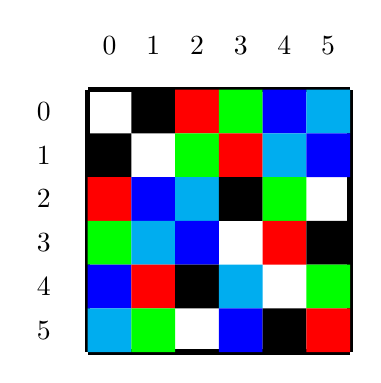
\begin{tikzpicture}[scale=0.1,line width = 2pt]
% box outline
\draw [] (0,3.33317) -- (0,-29.9988);
\draw [] (0,-29.9988) -- (33.332,-29.9988);
\draw [] (33.332,-29.9988) -- (33.332,3.33317);
\draw [] (33.332,3.33317) -- (0,3.33317);
\draw (-5.55533,0.555533) node{0};
\draw (-5.55533,-4.9998) node{1};
\draw (-5.55533,-10.5551) node{2};
\draw (-5.55533,-16.1105) node{3};
\draw (-5.55533,-21.6658) node{4};
\draw (-5.55533,-27.2211) node{5};
\draw (2.77767,8.88853) node{0};
\draw (8.333,8.88853) node{1};
\draw (13.8883,8.88853) node{2};
\draw (19.4437,8.88853) node{3};
\draw (24.999,8.88853) node{4};
\draw (30.5543,8.88853) node{5};
% 0_1
\fill [color=black, line width=0.1mm] (5.55533,3.33317) -- (5.55533,-2.22213) -- (11.1107,-2.22213) -- (11.1107,3.33317) -- (5.55533,3.33317);
% 0_2
\fill [color=red, line width=0.1mm] (11.1107,3.33317) -- (11.1107,-2.22213) -- (16.666,-2.22213) -- (16.666,3.33317) -- (11.1107,3.33317);
% 0_3
\fill [color=green, line width=0.1mm] (16.666,3.33317) -- (16.666,-2.22213) -- (22.2213,-2.22213) -- (22.2213,3.33317) -- (16.666,3.33317);
% 0_4
\fill [color=blue, line width=0.1mm] (22.2213,3.33317) -- (22.2213,-2.22213) -- (27.7767,-2.22213) -- (27.7767,3.33317) -- (22.2213,3.33317);
% 0_5
\fill [color=cyan, line width=0.1mm] (27.7767,3.33317) -- (27.7767,-2.22213) -- (33.332,-2.22213) -- (33.332,3.33317) -- (27.7767,3.33317);
% 1_0
\fill [color=black, line width=0.1mm] (0,-2.22213) -- (0,-7.77747) -- (5.55533,-7.77747) -- (5.55533,-2.22213) -- (0,-2.22213);
% 1_2
\fill [color=green, line width=0.1mm] (11.1107,-2.22213) -- (11.1107,-7.77747) -- (16.666,-7.77747) -- (16.666,-2.22213) -- (11.1107,-2.22213);
% 1_3
\fill [color=red, line width=0.1mm] (16.666,-2.22213) -- (16.666,-7.77747) -- (22.2213,-7.77747) -- (22.2213,-2.22213) -- (16.666,-2.22213);
% 1_4
\fill [color=cyan, line width=0.1mm] (22.2213,-2.22213) -- (22.2213,-7.77747) -- (27.7767,-7.77747) -- (27.7767,-2.22213) -- (22.2213,-2.22213);
% 1_5
\fill [color=blue, line width=0.1mm] (27.7767,-2.22213) -- (27.7767,-7.77747) -- (33.332,-7.77747) -- (33.332,-2.22213) -- (27.7767,-2.22213);
% 2_0
\fill [color=red, line width=0.1mm] (0,-7.77747) -- (0,-13.3328) -- (5.55533,-13.3328) -- (5.55533,-7.77747) -- (0,-7.77747);
% 2_1
\fill [color=blue, line width=0.1mm] (5.55533,-7.77747) -- (5.55533,-13.3328) -- (11.1107,-13.3328) -- (11.1107,-7.77747) -- (5.55533,-7.77747);
% 2_2
\fill [color=cyan, line width=0.1mm] (11.1107,-7.77747) -- (11.1107,-13.3328) -- (16.666,-13.3328) -- (16.666,-7.77747) -- (11.1107,-7.77747);
% 2_3
\fill [color=black, line width=0.1mm] (16.666,-7.77747) -- (16.666,-13.3328) -- (22.2213,-13.3328) -- (22.2213,-7.77747) -- (16.666,-7.77747);
% 2_4
\fill [color=green, line width=0.1mm] (22.2213,-7.77747) -- (22.2213,-13.3328) -- (27.7767,-13.3328) -- (27.7767,-7.77747) -- (22.2213,-7.77747);
% 3_0
\fill [color=green, line width=0.1mm] (0,-13.3328) -- (0,-18.8881) -- (5.55533,-18.8881) -- (5.55533,-13.3328) -- (0,-13.3328);
% 3_1
\fill [color=cyan, line width=0.1mm] (5.55533,-13.3328) -- (5.55533,-18.8881) -- (11.1107,-18.8881) -- (11.1107,-13.3328) -- (5.55533,-13.3328);
% 3_2
\fill [color=blue, line width=0.1mm] (11.1107,-13.3328) -- (11.1107,-18.8881) -- (16.666,-18.8881) -- (16.666,-13.3328) -- (11.1107,-13.3328);
% 3_4
\fill [color=red, line width=0.1mm] (22.2213,-13.3328) -- (22.2213,-18.8881) -- (27.7767,-18.8881) -- (27.7767,-13.3328) -- (22.2213,-13.3328);
% 3_5
\fill [color=black, line width=0.1mm] (27.7767,-13.3328) -- (27.7767,-18.8881) -- (33.332,-18.8881) -- (33.332,-13.3328) -- (27.7767,-13.3328);
% 4_0
\fill [color=blue, line width=0.1mm] (0,-18.8881) -- (0,-24.4435) -- (5.55533,-24.4435) -- (5.55533,-18.8881) -- (0,-18.8881);
% 4_1
\fill [color=red, line width=0.1mm] (5.55533,-18.8881) -- (5.55533,-24.4435) -- (11.1107,-24.4435) -- (11.1107,-18.8881) -- (5.55533,-18.8881);
% 4_2
\fill [color=black, line width=0.1mm] (11.1107,-18.8881) -- (11.1107,-24.4435) -- (16.666,-24.4435) -- (16.666,-18.8881) -- (11.1107,-18.8881);
% 4_3
\fill [color=cyan, line width=0.1mm] (16.666,-18.8881) -- (16.666,-24.4435) -- (22.2213,-24.4435) -- (22.2213,-18.8881) -- (16.666,-18.8881);
% 4_5
\fill [color=green, line width=0.1mm] (27.7767,-18.8881) -- (27.7767,-24.4435) -- (33.332,-24.4435) -- (33.332,-18.8881) -- (27.7767,-18.8881);
% 5_0
\fill [color=cyan, line width=0.1mm] (0,-24.4435) -- (0,-29.9988) -- (5.55533,-29.9988) -- (5.55533,-24.4435) -- (0,-24.4435);
% 5_1
\fill [color=green, line width=0.1mm] (5.55533,-24.4435) -- (5.55533,-29.9988) -- (11.1107,-29.9988) -- (11.1107,-24.4435) -- (5.55533,-24.4435);
% 5_3
\fill [color=blue, line width=0.1mm] (16.666,-24.4435) -- (16.666,-29.9988) -- (22.2213,-29.9988) -- (22.2213,-24.4435) -- (16.666,-24.4435);
% 5_4
\fill [color=black, line width=0.1mm] (22.2213,-24.4435) -- (22.2213,-29.9988) -- (27.7767,-29.9988) -- (27.7767,-24.4435) -- (22.2213,-24.4435);
% 5_5
\fill [color=red, line width=0.1mm] (27.7767,-24.4435) -- (27.7767,-29.9988) -- (33.332,-29.9988) -- (33.332,-24.4435) -- (27.7767,-24.4435);
\end{tikzpicture}
\end{document}
